\documentclass[11pt,oneside]{article}

\pdfminorversion=7
\usepackage{QuizStyle}

\hypersetup{
    pdftitle={20260930 Quiz for MATH200 Differential Equations},
    pdfauthor={Jungwoo Kim},
    pdfsubject={Quiz for MATH200 Differential Equations},
    pdfcreator={LaTeX}
}

\begin{document}

\quiztitle{20260930 Quiz}

\begin{problem}{2.7.3}
Consider the initial value problem
\[
    y'=1-t+2y,
    \qquad
    y(0)=1.
\]
\begin{problemsubparts}
    \item Find approximate values of the solution at $t=0.1,0.2,0.3,0.4$ using Euler's method with $h=0.1$.
    \item Repeat part (a) with $h=0.05$. Compare the results with those found in part (a).
    \item Repeat part (a) with $h=0.025$. Compare the results with those found in parts (a) and (b).
    \item Find the exact solution $y=\phi(t)$ of the initial value problem and evaluate $\phi(t)$ at $t=0.1,0.2,0.3,0.4$. Compare these values with the results of parts (a), (b), and (c).
\end{problemsubparts}
\end{problem}

\begin{solution}
\noindent\textup{(a)--(c)} For Euler's method,
\[
    t_n=nh,
    \qquad
    y_{n+1}=y_n+h(1-t_n+2y_n),
    \qquad
    y_0=1.
\]
Carrying out the recurrence gives
\[
\begin{array}{c@{\qquad}rrrr}
\toprule
h & y(0.1) & y(0.2) & y(0.3) & y(0.4) \\
\midrule
0.100 & 1.30000 & 1.65000 & 2.06000 & 2.54200 \\
0.050 & 1.31250 & 1.68013 & 2.11445 & 2.62949 \\
0.025 & 1.31938 & 1.69682 & 2.14482 & 2.67859 \\
\bottomrule
\end{array}
\]
Thus, for each listed value of $t$, the Euler approximations increase as the step size decreases.

\medskip
\noindent\textup{(d)} The differential equation can be written as
\[
    y'-2y=1-t.
\]
An integrating factor is $e^{-2t}$, so
\[
    (e^{-2t}y)'=(1-t)e^{-2t}.
\]
Hence
\[
    y=ce^{2t}+\frac{t}{2}-\frac14.
\]
Using $y(0)=1$ gives $c=5/4$, and therefore
\[
    \boxed{\phi(t)=\frac54e^{2t}+\frac{t}{2}-\frac14}.
\]
The corresponding exact values are
\[
\begin{array}{c@{\qquad}rrrr}
\toprule
 & \phi(0.1) & \phi(0.2) & \phi(0.3) & \phi(0.4) \\
\midrule
\text{Exact} & 1.32675 & 1.71478 & 2.17765 & 2.73193 \\
\bottomrule
\end{array}
\]
The Euler approximations move toward these exact values as $h$ decreases.
\end{solution}

\begin{problem}{2.8.2}
Transform the initial value problem
\[
    \frac{\dd y}{\dd t}=4-y^3,
    \qquad
    y(-1)=2,
\]
into an equivalent problem with the initial point at the origin.
\end{problem}

\begin{solution}
Set
\[
    s=t+1,
    \qquad
    w=y-2.
\]
Then the initial point $(t,y)=(-1,2)$ becomes $(s,w)=(0,0)$, and
\[
    \frac{\dd w}{\dd s}=\frac{\dd y}{\dd t}.
\]
Since $y=w+2$, the equivalent initial value problem is
\[
    \boxed{
        \frac{\dd w}{\dd s}=4-(w+2)^3,
        \qquad
        w(0)=0
    }.
\]
\end{solution}

\begin{problem}{2.8.7}
Let $\phi_0(t)=0$ and use the method of successive approximations to approximate the solution of
\[
    y'=2t^2+y^2,
    \qquad
    y(0)=0.
\]
\begin{problemsubparts}
    \item Calculate $\phi_1(t),\phi_2(t),\phi_3(t)$.
    \item Plot $\phi_1(t),\phi_2(t),\phi_3(t)$. Observe whether the iterates appear to be converging.
\end{problemsubparts}
\end{problem}

\begin{solution}
\noindent\textup{(a)} The successive approximations satisfy
\[
    \phi_{n+1}(t)
    =\int_0^t\left(2s^2+\phi_n(s)^2\right)\,\dd s.
\]
Thus
\[
    \phi_1(t)=\int_0^t2s^2\,\dd s
    =\frac23t^3,
\]
\[
    \phi_2(t)
    =\int_0^t\left(2s^2+\frac49s^6\right)\,\dd s
    =\frac23t^3+\frac4{63}t^7,
\]
and
\[
\begin{aligned}
    \phi_3(t)
    &=\int_0^t\left[2s^2+
        \left(\frac23s^3+\frac4{63}s^7\right)^2\right] \dd s \\
    &=\frac23t^3+\frac4{63}t^7
      +\frac{16}{2079}t^{11}
      +\frac{16}{59535}t^{15}.
\end{aligned}
\]
Hence
\[
    \boxed{
    \begin{aligned}
        \phi_1(t)&=\frac23t^3,\\
        \phi_2(t)&=\frac23t^3+\frac4{63}t^7,\\
        \phi_3(t)&=\frac23t^3+\frac4{63}t^7
        +\frac{16}{2079}t^{11}+\frac{16}{59535}t^{15}.
    \end{aligned}}
\]

\Needspace{23\baselineskip}
\medskip
\noindent\textup{(b)} The first three iterates are shown below.

\begin{center}
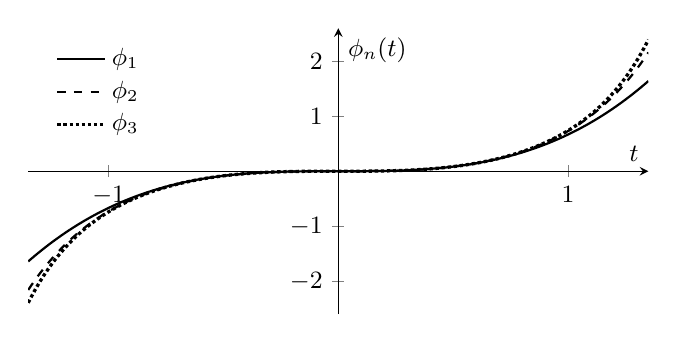
\begin{tikzpicture}
\begin{axis}[
    width=0.78\textwidth,
    height=0.43\textwidth,
    axis lines=middle,
    xmin=-1.35,
    xmax=1.35,
    ymin=-2.6,
    ymax=2.6,
    xlabel={$t$},
    ylabel={$\phi_n(t)$},
    xtick={-1,0,1},
    ytick={-2,-1,0,1,2},
    tick label style={font=\small},
    label style={font=\small},
    legend style={font=\small,draw=none,fill=none,at={(0.03,0.97)},anchor=north west},
    samples=400
]
    \addplot[black,thick,domain=-1.35:1.35] {(2/3)*x^3};
    \addlegendentry{$\phi_1$}
    \addplot[black,dashed,thick,domain=-1.35:1.35] {(2/3)*x^3+(4/63)*x^7};
    \addlegendentry{$\phi_2$}
    \addplot[black,densely dotted,very thick,domain=-1.35:1.35] {(2/3)*x^3+(4/63)*x^7+(16/2079)*x^11+(16/59535)*x^15};
    \addlegendentry{$\phi_3$}
\end{axis}
\end{tikzpicture}
\end{center}

Near the initial point, the successive iterates lie increasingly close to one another, which is consistent with convergence of the Picard iterates there.
\end{solution}

\begin{problem}{3.1.3}
Find the general solution of
\[
    12y''-y'-y=0.
\]
\end{problem}

\begin{solution}
The characteristic equation is
\[
    12r^2-r-1=0=(3r-1)(4r+1),
\]
so
\[
    r_1=\frac13,
    \qquad
    r_2=-\frac14.
\]
Therefore
\[
    \boxed{y=c_1e^{t/3}+c_2e^{-t/4}}.
\]
\end{solution}

\begin{problem}{3.1.4}
Find the general solution of
\[
    y''+6y'=0.
\]
\end{problem}

\begin{solution}
The characteristic equation is
\[
    r^2+6r=r(r+6)=0,
\]
with roots $r_1=0$ and $r_2=-6$. Hence
\[
    \boxed{y=c_1+c_2e^{-6t}}.
\]
\end{solution}

\begin{problem}{3.1.9}
Find the solution of the initial value problem
\[
    y''+3y'=0,
    \qquad
    y(0)=0,
    \qquad
    y'(0)=3.
\]
Sketch the graph of the solution and describe its behavior as $t$ increases.
\end{problem}

\begin{solution}
The characteristic equation is
\[
    r(r+3)=0,
\]
so the general solution is
\[
    y=c_1+c_2e^{-3t}.
\]
The initial conditions give
\[
    c_1+c_2=0,
    \qquad
    -3c_2=3,
\]
so $c_1=1$ and $c_2=-1$. Therefore
\[
    \boxed{y=1-e^{-3t}}.
\]

\Needspace{22\baselineskip}
The graph for $t\geq0$ is shown below; the dashed line is the horizontal asymptote $y=1$.

\begin{center}
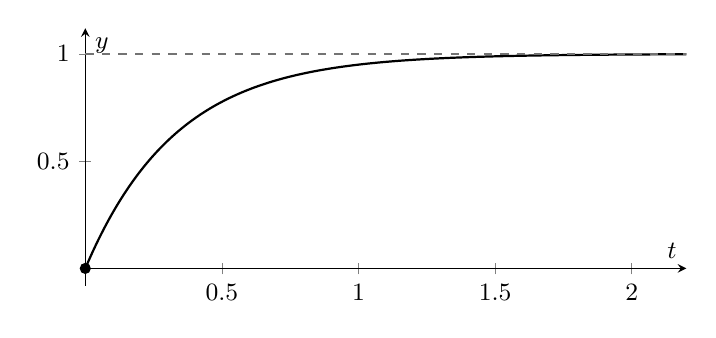
\begin{tikzpicture}
\begin{axis}[
    width=0.76\textwidth,
    height=0.40\textwidth,
    axis lines=middle,
    xmin=0,
    xmax=2.2,
    ymin=-0.08,
    ymax=1.12,
    xlabel={$t$},
    ylabel={$y$},
    xtick={0,0.5,1,1.5,2},
    ytick={0,0.5,1},
    tick label style={font=\small},
    label style={font=\small},
    clip=false,
    samples=300
]
    \addplot[black,thick,domain=0:2.2] {1-exp(-3*x)};
    \addplot[black!55,dashed] coordinates {(0,1) (2.2,1)};
    \addplot[only marks,mark=*,mark size=1.8pt,black] coordinates {(0,0)};
\end{axis}
\end{tikzpicture}
\end{center}

Since $e^{-3t}\to0$ as $t\to\infty$,
\[
    \boxed{y(t)\to1\quad\text{as }t\to\infty}.
\]
The solution increases from $0$ and approaches $1$ from below.
\end{solution}

\begin{problem}{3.2.7}
Determine the longest interval in which the initial value problem
\[
    t(t-4)y''+3ty'+5y=2,
    \qquad
    y(3)=0,
    \qquad
    y'(3)=-1
\]
is certain to have a unique twice-differentiable solution. Do not attempt to find the solution.
\end{problem}

\begin{solution}
Dividing by $t(t-4)$ gives
\[
    y''+\frac{3}{t-4}y'
    +\frac{5}{t(t-4)}y
    =\frac{2}{t(t-4)}.
\]
The coefficients are continuous except at $t=0$ and $t=4$. The largest open interval containing the initial point $t=3$ on which all coefficients are continuous is
\[
    \boxed{(0,4)}.
\]
By Theorem~3.2.1, the initial value problem has a unique twice-differentiable solution throughout this interval.
\end{solution}

\begin{problem}{3.2.18}
Consider the differential equation
\[
    y''-y'-2y=0.
\]
\begin{problemsubparts}
    \item Show that $y_1(t)=e^{-t}$ and $y_2(t)=e^{2t}$ form a fundamental set of solutions.
    \item Let
    \[
        y_3(t)=-2e^{2t},
        \qquad
        y_4(t)=y_1(t)+2y_2(t),
        \qquad
        y_5(t)=2y_1(t)-2y_3(t).
    \]
    Are $y_3(t)$, $y_4(t)$, and $y_5(t)$ also solutions of the differential equation?
    \item Determine whether each of the pairs $\{y_1(t),y_3(t)\}$ and $\{y_2(t),y_3(t)\}$ forms a fundamental set of solutions.
\end{problemsubparts}
\end{problem}

\begin{solution}
\noindent\textup{(a)} Direct substitution gives
\[
    y_1''-y_1'-2y_1=e^{-t}+e^{-t}-2e^{-t}=0
\]
and
\[
    y_2''-y_2'-2y_2=4e^{2t}-2e^{2t}-2e^{2t}=0,
\]
so both functions are solutions. Their Wronskian is
\[
\begin{aligned}
    W(y_1,y_2)(t)
    &=
    \begin{vmatrix}
        e^{-t} & e^{2t}\\
        -e^{-t} & 2e^{2t}
    \end{vmatrix}\\
    &=3e^t\neq0.
\end{aligned}
\]
Hence $y_1$ and $y_2$ form a fundamental set of solutions.

\medskip
\noindent\textup{(b)} Since $y_3=-2y_2$, $y_4=y_1+2y_2$, and
\[
    y_5=2y_1-2y_3=2y_1+4y_2,
\]
each is a linear combination of the solutions $y_1$ and $y_2$. By Theorem~3.2.2, all three are also solutions.

\medskip
\noindent\textup{(c)} Since $y_3=-2y_2$,
\[
    W(y_1,y_3)(t)=-2W(y_1,y_2)(t)=-6e^t\neq0,
\]
so
\[
    \boxed{\{y_1,y_3\}\text{ is a fundamental set}}.
\]
On the other hand, $y_2$ and $y_3$ are constant multiples of one another, so their Wronskian is zero. Thus
\[
    \boxed{\{y_2,y_3\}\text{ is not a fundamental set}}.
\]
\end{solution}

\begin{problem}{3.2.20}
Find the fundamental set of solutions specified by Theorem~3.2.5 for
\[
    y''+5y'+4y=0,
    \qquad
    t_0=1.
\]
\end{problem}

\begin{solution}
The characteristic equation is
\[
    r^2+5r+4=(r+1)(r+4)=0,
\]
so it is convenient to write the general solution as
\[
    y=Ae^{-(t-1)}+Be^{-4(t-1)}.
\]
By Theorem~3.2.5, $y_1$ is the solution satisfying
\[
    y_1(1)=1,
    \qquad
    y_1'(1)=0.
\]
Thus
\[
    A+B=1,
    \qquad
    -A-4B=0,
\]
which gives $A=4/3$ and $B=-1/3$. Hence
\[
    y_1(t)=-\frac13e^{-4(t-1)}+\frac43e^{-(t-1)}.
\]
Similarly, $y_2$ is the solution satisfying
\[
    y_2(1)=0,
    \qquad
    y_2'(1)=1.
\]
Then
\[
    A+B=0,
    \qquad
    -A-4B=1,
\]
so $A=1/3$ and $B=-1/3$. Therefore the specified fundamental set is
\[
    \boxed{
    \begin{aligned}
        y_1(t)&=-\frac13e^{-4(t-1)}+\frac43e^{-(t-1)},\\
        y_2(t)&=-\frac13e^{-4(t-1)}+\frac13e^{-(t-1)}.
    \end{aligned}}
\]
\end{solution}

\begin{problem}{3.3.6}
Find the general solution of
\[
    y''-2y'+8y=0.
\]
\end{problem}

\begin{solution}
The characteristic equation is
\[
    r^2-2r+8=0,
\]
with roots
\[
    r=1\pm i\sqrt7.
\]
Therefore
\[
    \boxed{
        y=c_1e^t\cos(\sqrt7\,t)
        +c_2e^t\sin(\sqrt7\,t)
    }.
\]
\end{solution}

\begin{problem}{3.3.13}
Find the solution of the initial value problem
\[
    y''-2y'+5y=0,
    \qquad
    y\left(\frac{\pi}{2}\right)=0,
    \qquad
    y'\left(\frac{\pi}{2}\right)=4.
\]
Sketch the graph of the solution and describe its behavior for increasing $t$.
\end{problem}

\begin{solution}
The characteristic equation is
\[
    r^2-2r+5=0,
\]
with roots $r=1\pm2i$. Hence
\[
    y=e^t(c_1\cos2t+c_2\sin2t).
\]
The first initial condition gives $c_1=0$. Thus
\[
    y=c_2e^t\sin2t,
\]
and
\[
    y'=c_2e^t(\sin2t+2\cos2t).
\]
Using $y'(\pi/2)=4$ gives
\[
    -2c_2e^{\pi/2}=4,
    \qquad
    c_2=-2e^{-\pi/2}.
\]
Therefore
\[
    \boxed{y=-2e^{t-\pi/2}\sin2t}.
\]

\Needspace{23\baselineskip}
The graph is shown below. The marked point is the initial point $(\pi/2,0)$.

\begin{center}
\begin{tikzpicture}
\begin{axis}[
    width=0.78\textwidth,
    height=0.43\textwidth,
    axis lines=middle,
    xmin=0,
    xmax=4,
    ymin=-25,
    ymax=25,
    xlabel={$t$},
    ylabel={$y$},
    xtick={0,1,2,3,4},
    ytick={-20,-10,0,10,20},
    tick label style={font=\small},
    label style={font=\small},
    clip=false,
    samples=500
]
    \addplot[black,thick,domain=0:4] {-2*exp(x-pi/2)*sin(deg(2*x))};
    \addplot[only marks,mark=*,mark size=1.8pt,black] coordinates {(1.5707963268,0)};
\end{axis}
\end{tikzpicture}
\end{center}

The trigonometric factor produces oscillation with period $\pi$, while the factor $e^{t-\pi/2}$ makes the amplitude grow exponentially. Thus the solution is a
\[
    \boxed{\text{growing oscillation}}.
\]
\end{solution}

\begin{problem}{3.4.4}
Find the general solution of
\[
    4y''-12y'+9y=0.
\]
\end{problem}

\begin{solution}
The characteristic equation is
\[
    4r^2-12r+9=(2r-3)^2=0,
\]
so $r=3/2$ is a repeated root. Therefore
\[
    \boxed{y=c_1e^{3t/2}+c_2te^{3t/2}}.
\]
\end{solution}

\begin{problem}{3.4.19}
Use the method of reduction of order to find a second solution of
\[
    t^2y''+ty'-4y=0,
    \qquad
    t>0,
\]
given that $y_1(t)=t^2$ is one solution.
\end{problem}

\begin{solution}
Set
\[
    y=v(t)y_1(t)=v(t)t^2.
\]
Then
\[
    y'=v't^2+2vt,
    \qquad
    y''=v''t^2+4v't+2v.
\]
Substitution into the differential equation gives
\[
    t^4v''+5t^3v'=0.
\]
Since $t>0$, this reduces to
\[
    tv''+5v'=0.
\]
Let $w=v'$. Then
\[
    tw'+5w=0,
\]
so
\[
    \frac{w'}{w}=-\frac5t.
\]
Hence
\[
    w=ct^{-5},
    \qquad
    v=-\frac{c}{4}t^{-4}+k.
\]
Therefore
\[
    y=vt^2=-\frac{c}{4}t^{-2}+kt^2.
\]
The term $kt^2$ is a multiple of the known solution $y_1$, while $t^{-2}$ is not a constant multiple of $t^2$. Thus an independent second solution is
\[
    \boxed{y_2(t)=t^{-2}}.
\]
\end{solution}

\end{document}
